\section{The Radon transform}
\label{sec:Radon}
The Radon transform (RT) is a mathematical transformation of an image devised to reveal internal properties of an object such as structure. The method was originally devised by Johann Radon in 1917 \citep{radon1917determination}. Since then the technique has been applied to many fields, including various branches of astronomy including microwave, radio and x-ray applications. \citet{deans2007radon} describes many of these applications, and also includes an English translation of Radon's original German text. In a more recent treatment  \citet{7910dc8d5b654c90ac4bc94c67d06f01} describes the application of the RT in the field of digital signal processing and presents algorithms for its implementation. For our purposes \cite{2018MNRAS.480.2217S} describe the application of the Radon Transform to galaxy kinematic studies.  

\begin{figure}[h]
    \centering
    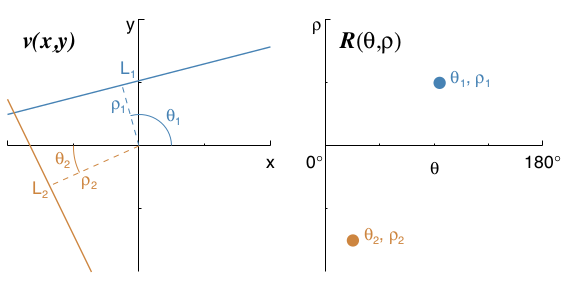
\includegraphics[width=\columnwidth]{images/RadonPlots/Radon-transform-Stark.png}
    \caption{The Radon transform: the figure illustrates the Radon transform and its coordinate system as described in \citet{2018MNRAS.480.2217S}. Line integrals across an image are calculated along all possible lines, parameterised by the coordinates [$\theta$, $\rho$], that cross the 2D function v(x, y). Two examples are shown in the left-hand panel, where the integrals are calculated over the solid lines, L$_1$ and L$_2$, which are perpendicular to the [$\theta, \rho$] vectors and mapped to the points $\theta_1$, $\rho_1$ and $\theta_2$, $\rho_2$ in [$\theta$, $\rho$] parameter space in the right-hand panel. In the Radon transform coordinate system, $\theta$ ranges from 0 to 180 $\deg$ while $\rho$ ranges from $-\infty$ to $\infty$  such that a position below the x-axis corresponds to $\rho < 0$.}
    \label{fig:RadonTransform}
\end{figure}

\citet{2018MNRAS.480.2217S} have applied the Radon transform technique to stellar and gas velocity fields obtained from the MaNGA integral field survey in order to quantify radial variations in the kinematic position angles of galaxies (PA$_k$) using the Radon transform method \citep[see e.g.][]{radon1917determination, 7910dc8d5b654c90ac4bc94c67d06f01}. 
The Radon Transform, $R$, is defined as

\begin{equation}
    \label{eqn:radon}
    R(\rho,\theta)=\int_{L}{v(x,y)\, \diff l},
\end{equation}

where $v(x,y)$ is a 2D velocity field defined in Cartesian coordinates and $\int_{L}$ is the line integral at transform sky-plane polar coordinates ($\rho,\theta$). This transform is illustrated graphically in Fig. \ref{fig:RadonTransform} where lines through an image in 2D velocity space are mapped to a series of points in Radon transform [$\theta,\rho$] space by means of line integrals at various angles about the velocity space axes, and at various distances offset from the velocity space origin. 

\citet{2018MNRAS.480.2217S} apply a modification to the Radon transform, to obtain the \textit{Absolute} Radon Transform, as defined in Eqn. (\ref{eqn:radon}), by taking the integral of the absolute values of the velocity field difference of each point $v(x_i,y_i)$ and the mean of all values along the line segment.

\begin{equation}
    \label{eqn:radon_absolute}
    R_A=\int{| v(x,y) - \langle v(x,y) \rangle | \, \diff l}.
\end{equation}

There is a further variants to the Absolute Radon Transform described by \citet{2018MNRAS.480.2217S} called the \textit{bounded}, or aperture restricted, Radon transform, R$_{AB}$. Briefly, R$_{AB}$ involves placing integration limits $(\pm{r_{ap}})$, known as the aperture, on the integral of Eqn. \ref{eqn:radon_absolute} in order to limit the number of spaxels across a velocity map that will be used in the integration.

These are discussed extensively in their Section XX and illustrated in their Figure 2.


\citet{2018MNRAS.480.2217S} have developed a set of IDL (Interactive Data Language) algorithms to perform the Radon transform on an input array representing a velocity field. The IDL code procedures we use in this work is named \texttt{ds\_radon.pro}.

An example of the graphical output of the Radon transform code \texttt{ds\_radon.pro} as applied to a synthetic velocity field is shown in Fig. \ref{fig:Radon}.

\begin{figure}
    \centering
   	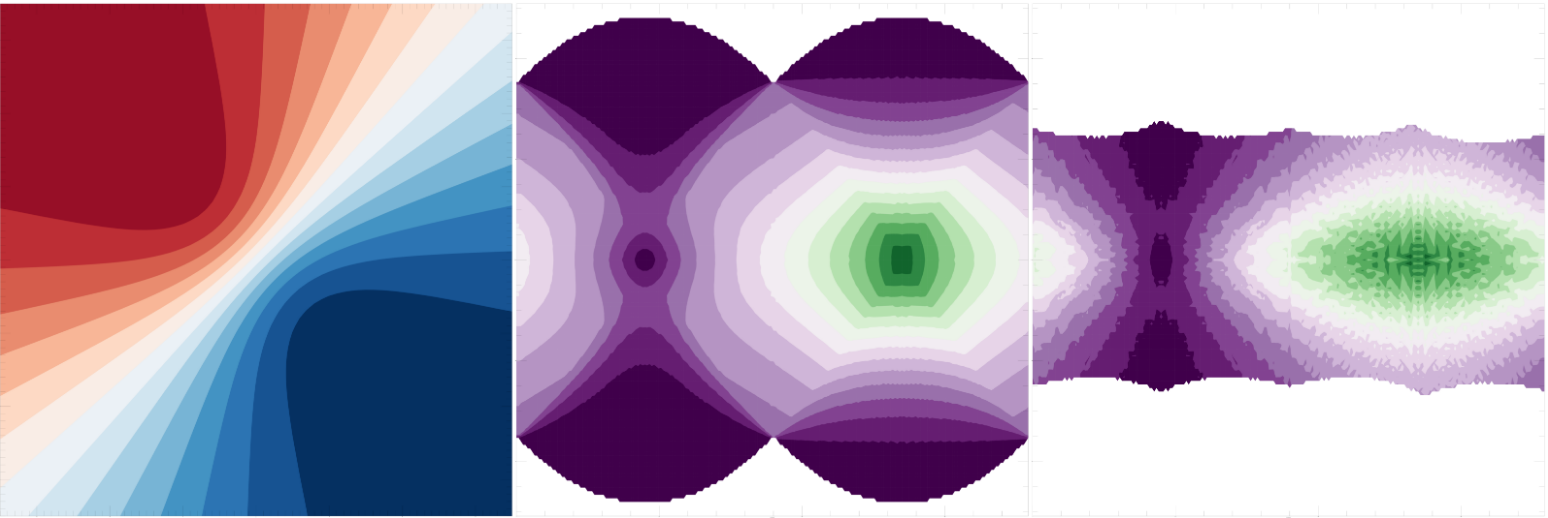
\includegraphics[width=\columnwidth]{images/RadonPlots/example.png}
    \caption{Model Radon transform plots as described in \citet{2018MNRAS.480.2217S}. The left panel shows a synthetic uniform velocity field model, the middle panel shows the the absolute Radon transform of the velocity field and the right panel shows the aperture-restricted absolute transform. We are concerned with the latter, the absolute aperture-restricted  Radon transform of stellar and gas velocity fields in this work.}
    \label{fig:Radon}
\end{figure}

Following \citet{2018MNRAS.480.2217S} we will demonstrate the application of the Radon transform to stellar and gas velocity field data obtained from the SDSS-IV MaNGA integral field survey for a selection of CPSB and RPSB galaxies.  

[This is new method of characterising position angles and how the $\Delta$PA varies within galaxies.]


\begin{figure}
    \centering
   	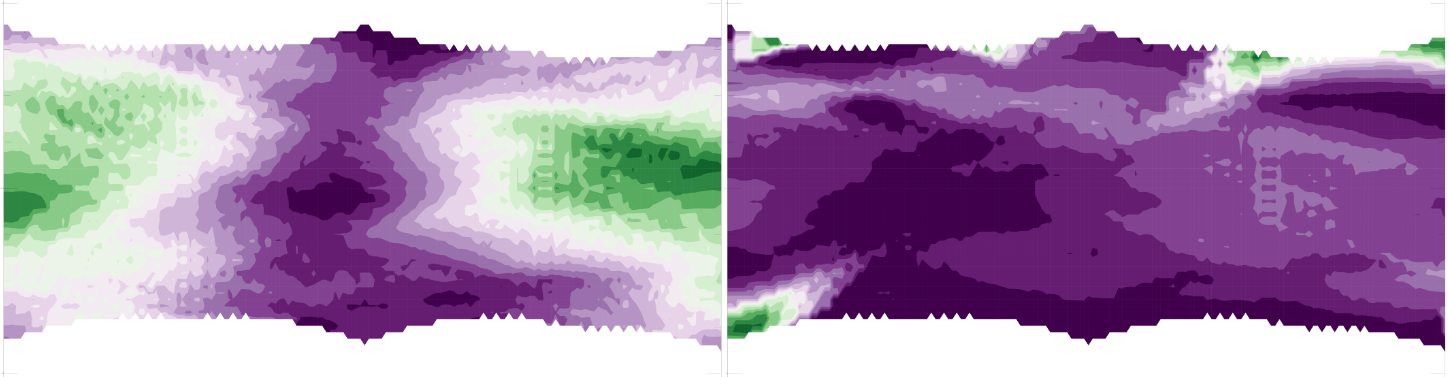
\includegraphics[width=\columnwidth]{images/RadonPlots/RT-snips/CPSB-8313-6101-RT-snip.png}
    \caption{Radon transform plots of the stellar velocity (left panel) and gas velocity (right) fields of CPSB of MaNGA PLATEIFU 8131-6101}
    \label{fig:RT_8131-6101}
\end{figure}



\begin{figure}
    \centering
    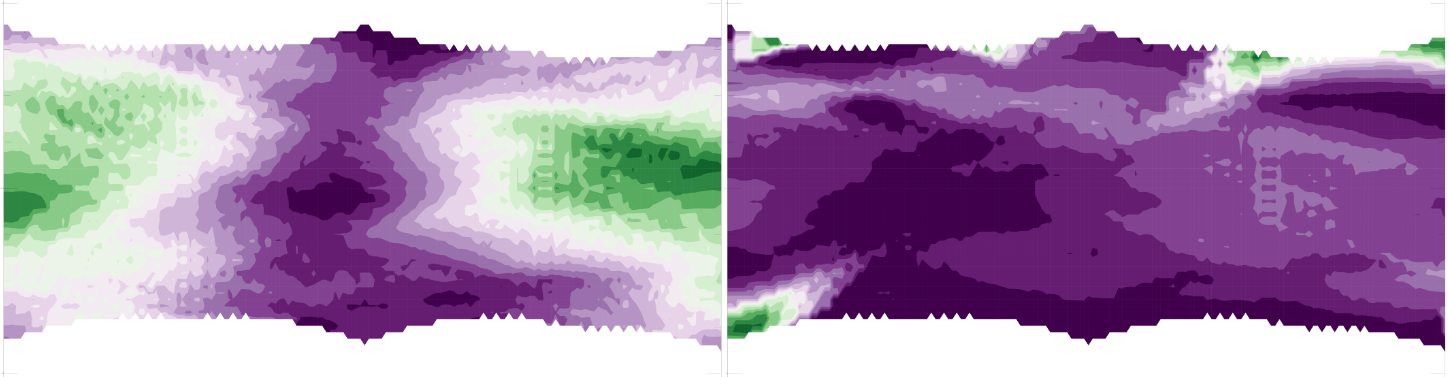
\includegraphics[width=\columnwidth]{images/RadonPlots/RT-snips/CPSB-8313-6101-RT-snip.png}
    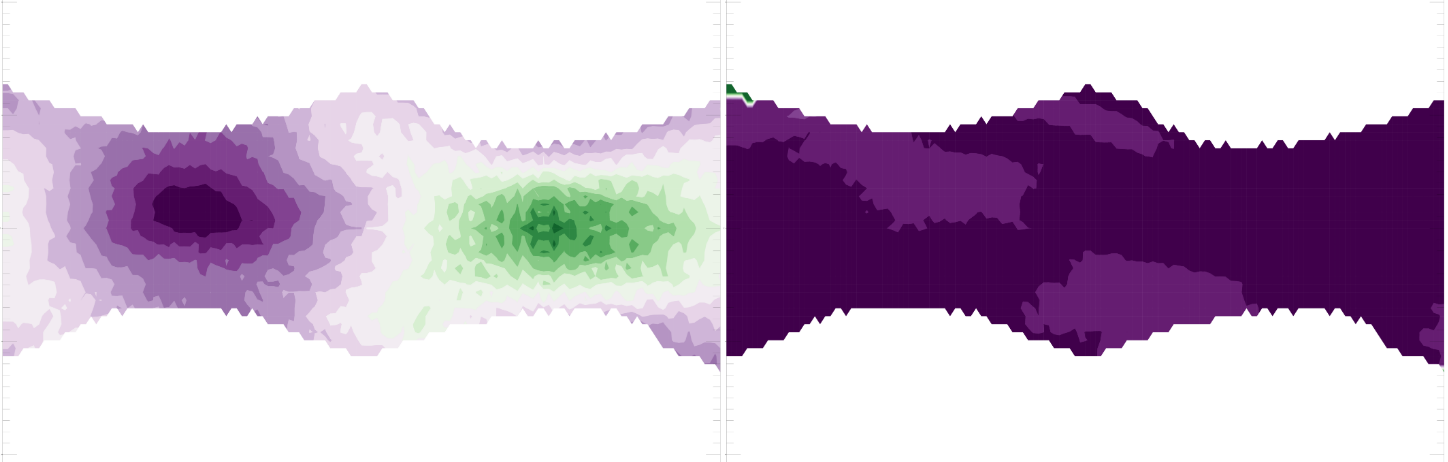
\includegraphics[width=\columnwidth]{images/RadonPlots/RT-snips/CPSB-9494-3701-RT-snip.png}
    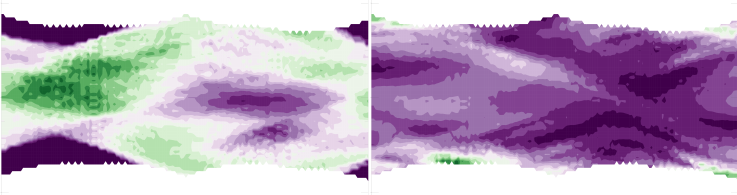
\includegraphics[width=\columnwidth]{images/RadonPlots/RT-snips/CPSB-8398-6102-RT-snip.png}
    \caption{CPSBs: Radon transforms of stellar velocity and gas velocity maps. From the top CPSB-8313-6101, CPSB-9404-3710 and CPSB -8398-6103}
    \label{fig:CPSB-RTs}
\end{figure}

\begin{figure}
    \centering
    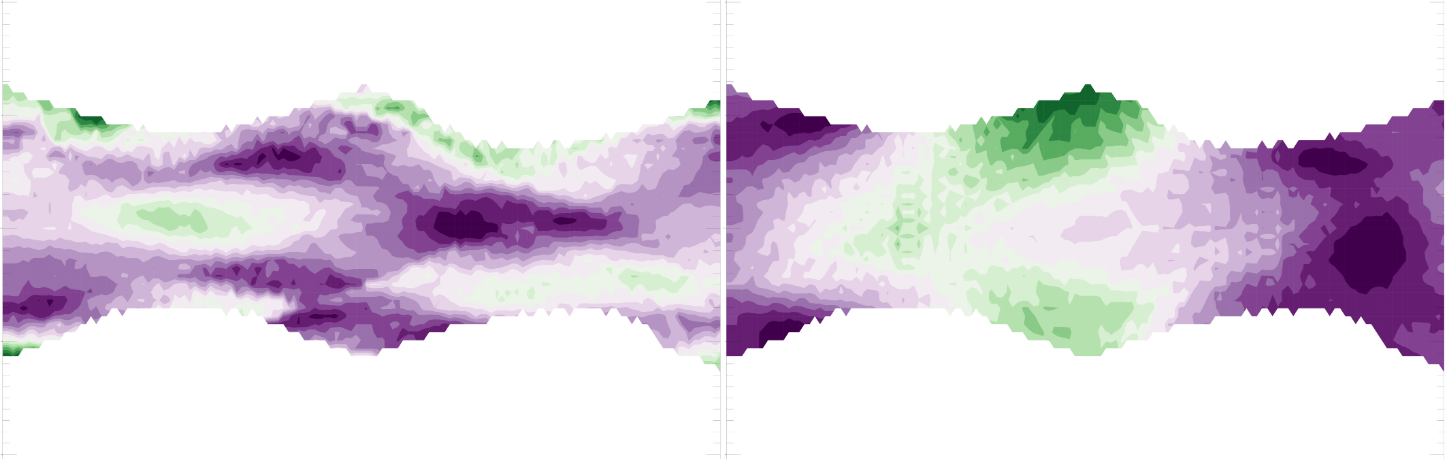
\includegraphics[width=\columnwidth]{images/RadonPlots/RT-snips/RPSB-9872-3701-RT-snip.png}
    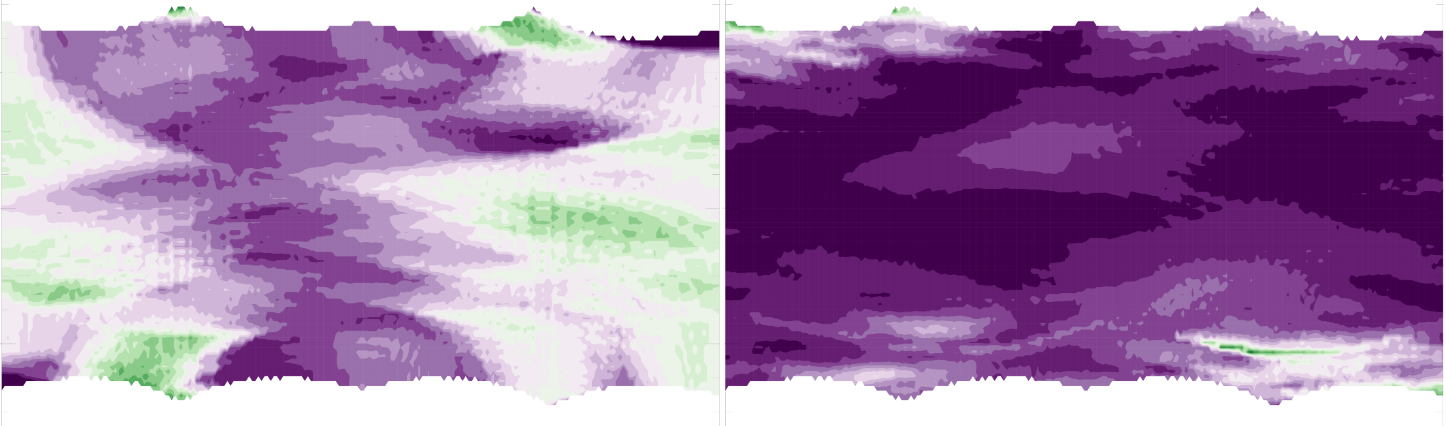
\includegraphics[width=\columnwidth]{images/RadonPlots/RT-snips/RPSB-8932-12704-RT-snip.png}
    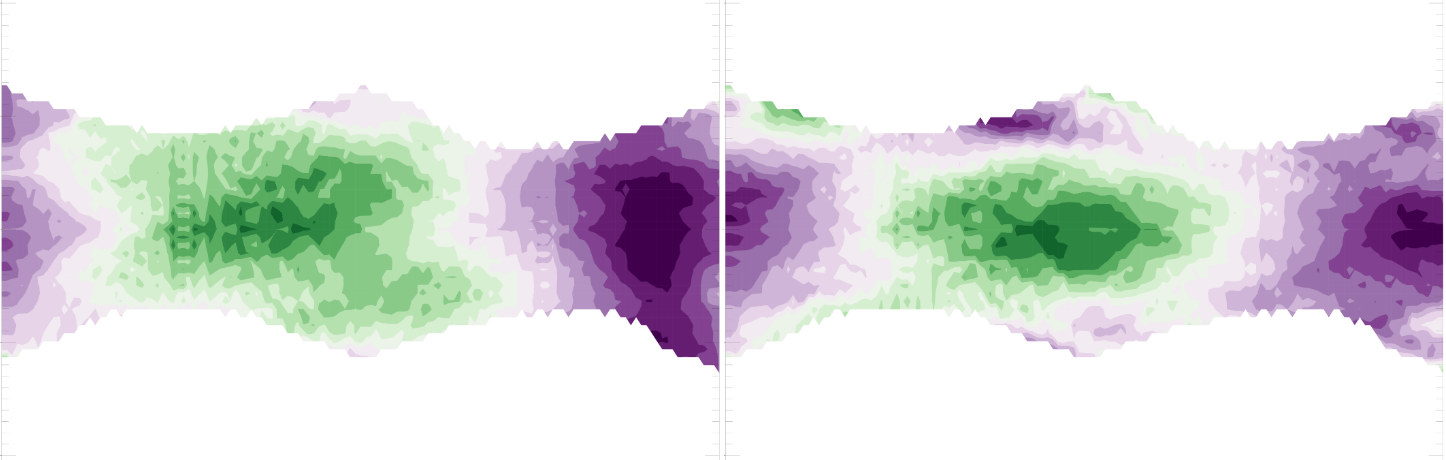
\includegraphics[width=\columnwidth]{images/RadonPlots/RT-snips/RPSB-8554-3701-RT-snip.png}
    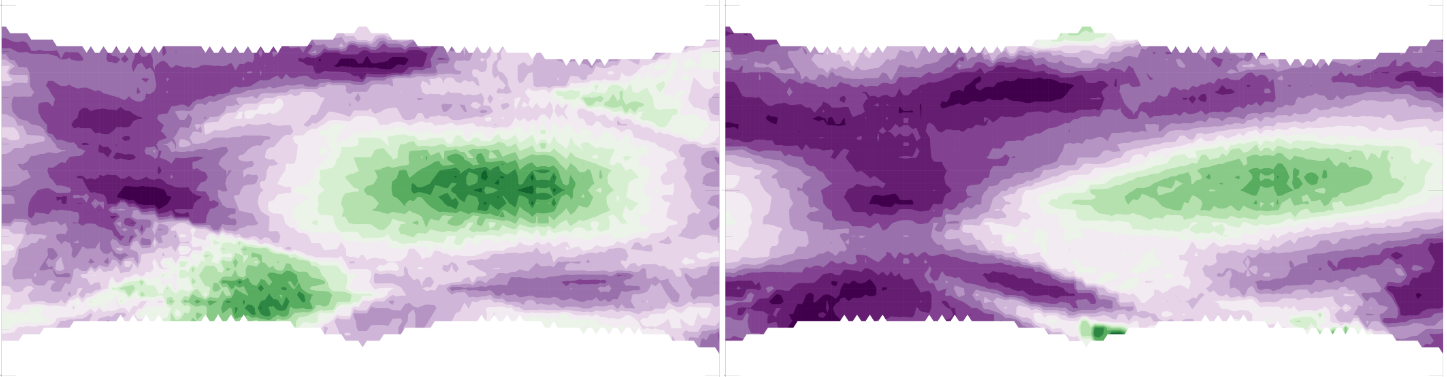
\includegraphics[width=\columnwidth]{images/RadonPlots/RT-snips/RPSB-8323-6103-RT-snip.png}
    \caption{Caption}
    \label{fig:RPSB-RTs}
\end{figure}